\documentclass[a4paper,12pt]{article}
\usepackage[margin=0.25in]{geometry}
\usepackage{amsmath,amssymb,graphicx,ulem,fancyhdr,fix-cm,xcolor,soul}
\usepackage[utf8]{inputenc}
\usepackage[english]{babel}
\usepackage{xcolor}
\usepackage{lastpage}
\usepackage[english]{babel}
\usepackage{titlesec}
\usepackage{enumitem}

\titleformat{\section}[runin]
{\normalfont\Large\bfseries}{\thesection}{}{}
\definecolor{background}{rgb}{1,1,0.92}
\pagenumbering{arabic}
\graphicspath{ {./images/} }
\setlength\headheight{110pt} 
\pagestyle{fancy}


%document variables 
\newcommand{\SheetNum}{Sheet 2 }
\newcommand{\SheetName}{Convergence \& Bisection }
\newcommand{\CourseCode}{CSE 213 }
\newcommand{\CourseName}{Numerical Analysis}



\begin{document}
\large
\section*{}%Coverpage
%cover Page,w/ university logo
 \pagecolor{background}
 \fancyhead[R]{ 
\includegraphics[width=12cm]{logo.png}}
 \fancyhead[L]{\fontsize{15}{20} \selectfont \textbf{\CourseCode - \CourseName\\ Spring '22\\ \ \\}}	
	\begin{center}
	\vspace*{6cm}
	\fontsize{40}{60} \selectfont \SheetNum - \SheetName \\
	\fontsize{30}{40}\selectfont \CourseCode - \CourseName \\
	\fontsize{28}{35}\selectfont 120200033 \qquad \ CSE Section 01\\
	\fontsize{25}{30}\selectfont Ahmad Mongy Saad Aboelnaga\\
	\fontsize{20}{25}\selectfont Ahmad.Aboelnaga@ejust.edu.eg	
	\newpage
	\end{center}
	\addtolength{\topmargin}{-.75in}
	\fancyhead[R]{\Large \textbf{\SheetNum}}
	 \fancyhead[L]{\fontsize{18}{20} \selectfont \CourseCode - \CourseName, Spring '22}
\section*{\LARGE Question 1:}{ \LARGE \textbf{Rate of Convergence and Order of Conver-\\[0.2cm] gence}}
\begin{enumerate}[label=(\alph*)]
\item  Determine the rate of convergence of the following sequences:
\begin{enumerate}[label=(\roman*)]
\item $x_n = 1 + (\dfrac{1}{2})^n$\\
{\color{blue}{\Large Solution:}  $x_{n \to \infty} = 1, \dfrac{\|x_{n+1}-x_\infty\|}{\|x_n-x_\infty\|} = \dfrac{\left(\dfrac{1}{2}\right)^{n+1}}{\left(\dfrac{1}{2}\right)^n} = \dfrac{1}{2} , \; O({ 1 \over 2}^n)$\\[0.2cm] \text{ (converges linearly, p=1, $0<k =0.5<1$)}\color{black}}\\[0.4cm]
\item $x_n = 1 + (\dfrac{1}{n})^n$\\
{\color{blue}{\Large Solution:}  $x_{n \to \infty} = 1, \dfrac{\|x_{n+1}-x_\infty\|}{\|x_n-x_\infty\|} = \dfrac{\left(\dfrac{1}{n}\right)^{n+1}}{\left(\dfrac{1}{n}\right)^n} = \dfrac{1}{n} \rightarrow \lim_{n \to \infty} \dfrac{1}{n} =0, \; O({ 1 \over n}^n) $\\ \text{ (converges super-linearly, p=1, $k=0$)}\color{black}}
\end{enumerate}
\item Suppose you apply an iterative method and obtain the following errors from the first four steps: $10^{-2}, 10^{-4}, 10^{-6}, 10^{-8}$, .... How would you characterize the order of convergence of this method?
\begin{enumerate}[label=(\Alph*)]
\item {\color{blue} Linear $\qquad  \Rightarrow \| e_{n+1}\| \approx 10^{-2} \|e_{n}\| \Rightarrow $ \begin{tabular}{|c|c|}
\hline 
$e_{n}$ & k= $\|e_{n+1}\|/\|e_{n}\|$ \\ 
\hline 
$10^{-2}$ & --- \\ 
\hline 
$10^{-4}$ & $10^{-2}$ \\ 
\hline 
$10^{-6}$ & $10^{-2}$ \\ 
\hline 
$10^{-8}$ & $10^{-2}$ \\ 
\hline 
\end{tabular}}
\item Super-linear
\item Quadratic
\item Faster than Quadratic
\end{enumerate}
\newpage
\item Suppose you apply an iterative method and obtain the following errors from the first four steps: $10^{-2}, 10^{-4}, 10^{-8}, 10^{-16}$, .... How would you characterize the order of convergence of this method?
\begin{enumerate}[label=(\Alph*)]
\item Linear
\item Super-linear
\item {\color{blue} Quadratic $\qquad  \Rightarrow \| e_{n+1}\| \approx 1 \|e_{n}\|^2  \Rightarrow $\begin{tabular}{|c|c|}
\hline 
$e_{n}$ & k= $\|e_{n+1}\|/\|e_{n}^2\|$ \\ 
\hline 
$10^{-2}$ & --- \\ 
\hline 
$10^{-4}$ & $1$ \\ 
\hline 
$10^{-8}$ & $1$ \\ 
\hline 
$10^{-16}$ & $1$ \\ 
\hline 
\end{tabular}}
\item Faster than Quadratic
\end{enumerate}
\item Limits Involving Continuous Functions Defined on Convergent Sequences: Determine whether the sequence $\lim_{n \to \infty } \cos (\frac{3}{n^2})$	 converges. If it converges, find its limit.\\
{\color{blue}{\Large Solution:} $\lim_{n \to \infty } \cos (\frac{3}{n^2})\rightarrow \lim_{n \to \infty } \cos (0) = 1$, The sequence converges with limit =1 }
\item Rate of convergence of functions. Definition. Let f be a function defined on the interval (a,b) that contains x=0, and suppose $\lim_{x \to 0 } f(x) = L$. If there exists a function g for which $\lim_{x \to 0 } g(x) = 0$ and a positive constant K such that \[ |f(x) -L | \le  K|g(x)| \] for all sufficiently small values of x, then f(x) is said to converge to L with rate of convergence O(g(x)).\\
Find the Rate of convergence of the following function as $h \rightarrow 0 : \lim_{h \to 0} {sin(h)\over h} =1$\\
{\color{blue}{\Large Solution:} $\lim_{h \to 0} {sin(h)\over h} =1 \rightarrow \sin(h) =h - \dfrac{h^3}{ 3!} \cdots ,\\ \rightarrow \lim_{h \to 0} \dfrac{sin(h)}{h} = \lim_{h \to 0} \dfrac{h - {h^3 \over 3!} \cdots }{h} =\lim_{h \to 0} 1-\dfrac{h^2}{6} \cdots \\ \therefore \| \lim_{h \to 0} \dfrac{sin(h)}{h} - 1 \| \le \dfrac{1}{6} h^2\\ k = \dfrac{1}{6},\; O(h^2) $}
\item Determine the order of convergence of the sequence generated by the iterative algorithm used to find$\sqrt{a}$ , where a is a positive real number using the following recursive formula: \[x_{n+1} = {1 \over 2} (x_n + {a \over x_n}) \] To accomplish this we must be able to compare the error in the $(n+1)\textsuperscript{th}$ term in the sequence $x_{n+1} - \sqrt{a}$ with error in the n\textsuperscript{th}, $x_{n} - \sqrt{a}$
\newpage
\color{blue}{\Large Solution:}
\begin{align*}
x_{n+1} - \sqrt{a} &= {1 \over 2} (x_n + {a \over x_n})\\ &= {1 \over 2}\left(\dfrac{x_n^2+a}{x_n}\right) - \sqrt{a} \\ &= {1 \over 2x_n}\left(x_n^2 +a -2x_n \sqrt{a} \right) \\ &=\dfrac{\left( x_n -\sqrt{a} \right)^2}{2x_n}\\ \therefore \lim_{n \to \infty} \dfrac{\|x_{n+1} - \sqrt{a}\|}{\|x_{n} - \sqrt{a}\|^p} &= \dfrac{\left( x_n -\sqrt{a} \right)^2}{2x_n(\|x_{n} - \sqrt{a}\|^p)} , \textbf{ with } p =2 \\  \lim_{n \to \infty} \dfrac{1}{2x_n} &= \dfrac{1}{2\sqrt{a}} \therefore \textbf{ The order of convergence is quadratic }
\end{align*}
\end{enumerate}

\section*{\LARGE Question 2:}{ \LARGE \textbf{\emph {Bisection Method}}\Large { for root finding– Textbook (9\textsuperscript{th}edition) – Problem Set 2.1 (Page 54). Answers should be given in a tabular form (as in the lecture slides).}}\\[0.5cm]
2. Let $f(x) = 3(x+1)(x-{1 \over 2})(x-1).$ Use the bisection method on the following intervals to find p\textsubscript{3}\\
\begin{enumerate}[label=(\alph*)]
\item $\left[-2,1.5\right]$ \textbf{\qquad \qquad \qquad \qquad \qquad \qquad \quad  Answers: a. -0.6875}\\
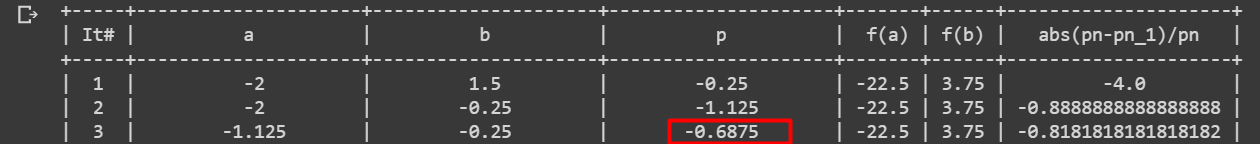
\includegraphics[scale=0.78]{Q2 2.a.png}
\item $\left[-1.25,2.5\right]$ \textbf{\qquad \qquad \qquad \qquad \qquad \qquad \quad  Answers: b. 1.09375}\\
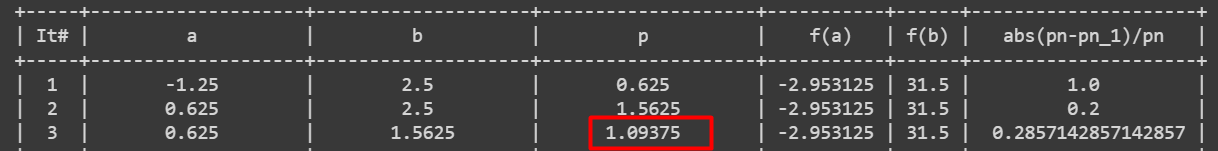
\includegraphics[scale=0.78]{Q2 2.b.png}
\end{enumerate}
\newpage
5. use the bisection method to find solutions accurate to within $10^{-5}$ for the following problems.
\begin{enumerate}[label=(\alph*)]
\item $x-2^{-x} = 0 \qquad \qquad \qquad $ for $\; 0\le x \le 1$ \textbf{\quad Answers: a. p17= 0.641182}\\
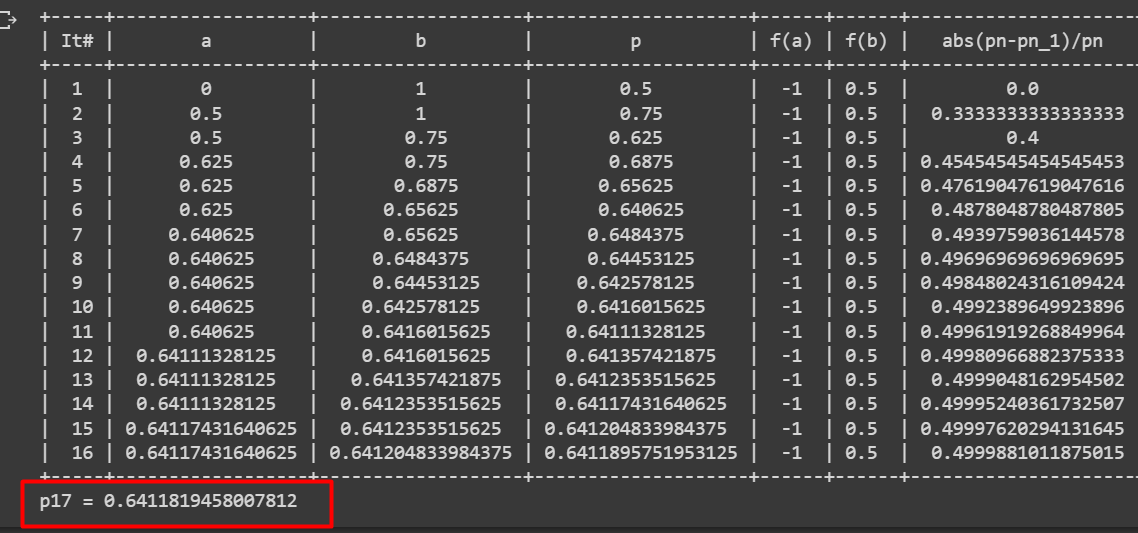
\includegraphics[scale=0.79]{Q2 5.a.png}

\item $e^{x} -x^{2} + 3x -2  = 0 \, \qquad $ for $\; 0\le x \le 1$ \textbf{\quad Answers: b. p17= 0.257530}\\
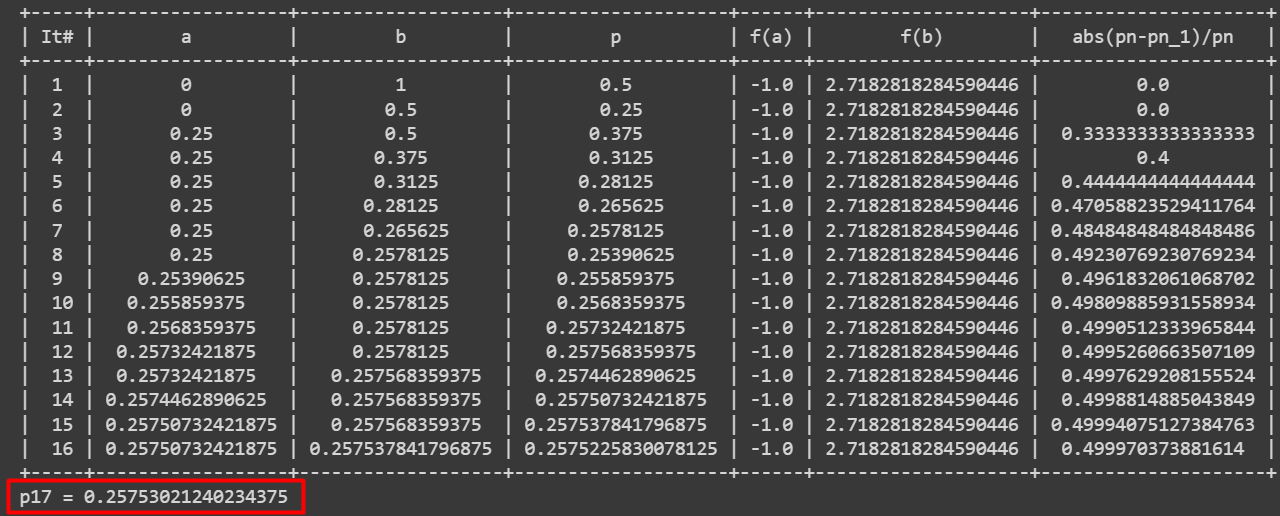
\includegraphics[scale=0.72]{Q2 5.b.png}
\end{enumerate}

 Tools used in creating this document:
 \begin{itemize}
 \item Texmaker 5.0.4
 \item Spyder IDE 5.1.5 with python 3.8.5
\end{itemize}  
 
 \copyright All questions in this file has been adapted from the sheet provided by the course instructor, I have only reorganized the sheet and attempted to answer it. Please do not share without the permission of the owner.\\
\color{blue}Ahmad.Aboelnaga@ejust.edu.eg\\
ID:120200033, CSE01
 
  
\end{document}			
